\chapter{Gestaltungslösungen implementieren}
\label{chapter:implementation}

Im vorherigen Schritt wurden konkrete Nutzungsanforderungen herausgearbeitet
und Ideen für passende Gestaltungslösungen formuliert. Das folgende
Kapitel soll sich mit der praktischen Umsetzung der Anforderungen beschäftigen.
Dieser Prozess entspricht dem dritten Schritt \textit{Gestaltungslösungen
    entwickeln, die die Nutzungsanforderungen erfüllen} des Designzyklus im Human
Centered Design nach ISO 9241 \cite{ISO9241}.

\section{Kundenwünsche und technische Machbarkeit}
Auch wenn im Human Centered Design immer die Nutzenden und nicht das technische
System im Fokus stehen sollte, kommt man nicht drumherum, die technischen
Details genauer zu betrachten. Dadurch ist es ganz besonders wichtig, in dieser
Phase die Bedürfnisse und Erwartungen der Nutzenden nicht aus den Augen zu
verlieren. Eine klare und intuitive Schnittstelle für die Nutzenden sollte in
diesem Prozess eine höhere Priorität einnehmen als eine Lösung, die technisch
am einfachsten umzusetzen ist. K. Holtzblatt verwendet hier den Begriff
\textit{Kohärenz} und meint damit, dass sich ein System für den Nutzer so
zusammenhängend und natürlich wie möglich anfühlen soll: \glqq{}The challenge
is to keep the system work model coherent, so that it supports the users and
fits with their expectations while extending and transforming their work
practice as prescribed by the vision.\grqq{} \cite{contextualDesign}
Gleichzeitig müssen alle Lösungsansätze natürlich auch tatsächlich programmiert
werden können. Hierbei kann nicht ignoriert werden, dass viele externe Faktoren
die Machbarkeit bestimmter Lösungskonzepte in der Praxis einschränken. G.A. Boy
erwähnt in \textit{The Handbook of Human-Machine Interaction} einige dieser
Faktoren: \glqq{}Design work is often constrained by various external factors
in the development organization and the marketplace (policies, standards,
competitive products, past and planned products, schedules, resource
budgets).\grqq \cite{HMI-HCD} So ermöglichen verwendete Programmiersprachen,
eingesetzte Frameworks und bereits existierende Softwareteile es, bestimmte
Konzepte sehr elegant umzusetzen. Andere Gestaltungsideen sind, beschränkt
durch äußere Faktoren, unter Umständen gar nicht realisierbar \cite{HMI-HCD}.

\section{Technische Grundlagen Stubegru}
In dem konkreten Fall des Moduls zur Terminvergabe für die Studienberatung ist
hier ein wichtiger Gesichtspunkt, dass es sich um ein Modul innerhalb eines
bereits bestehenden Softwarepakets handelt. \gls{Tech-Stack},
Programmiersprache und Schnittstellen zu anderen Modulen sind hier bereits
vorgeben und können nicht allein durch die Wünsche der Nutzenden geformt
werden.

\subsection*{Tech Stack}
Im Folgenden sollen nun die technischen Gegebenheiten und Grundlagen der
Software Stubegru vorgestellt werden. Das neue System zur Terminvereinbarung
muss sich als Modul in das Softwarepaket Stubegru einbinden lassen und somit
einige Standards und Schnittstellen der Software zur Verfügung stellen.

Die Software Stubegru ist webbasiert und wird über einen Browser aufgerufen.
Dementsprechend sind die verwendeten Technologien im Frontend \gls{Html},
\gls{Css} und \gls{Javascript}. Die Kommunikation mit dem Backend wird durch
asynchrone Requests umgesetzt, die durch Javascript Methoden initiiert werden.
Das Backend besteht aus vielen einzelnen \gls{Php} Dateien, welche die per
\gls{Http} übermittelten Daten auslesen und aufarbeiten. Als Datenbank kommt
eine relationale \gls{MySQL} Datenbank zum Einsatz, die von den Php Skripten
über \gls{PDO} angesprochen wird. Die abgerufenen Daten der Php Skripte werden,
als \gls{JSON} codiert zurück an das Frontend geschickt und dort von Javascript
Methoden weiterverarbeitet. Mithilfe der Javascript Library \gls{jQuery} werden
die entsprechenden Elemente im \gls{Document-Object-Model} angepasst und somit
für den Nutzenden grafisch dargestellt. Um den Nutzenden eine einheitliche und
vertraute Nutzungsoberfläche zu bieten, kommt das Framework \gls{Bootstrap} zum
Einsatz.

Das Softwarepaket Stubegru ist grundlegend modular aufgebaut, sodass für jede
Funktionalität oder jeden Prozess ein eigenes Modul programmiert wird, das
genau diese Aufgabe übernimmt. Jedes Modul besteht aus den entsprechenden
Anzeigeelementen, die in einer Html Datei formuliert werden. Des weiteren aus
grafischen Designregeln, die als CSS Datei angelegt werden und der eigentlichen
Logik, die in Javascript implementiert werden muss. Im Modul zur
Terminvereinbarung kommt zusätzlich die Javascript Library \gls{fullcalendar}
zum Einsatz. Diese bietet eine einfache Schnittstelle, um Termindaten in einer
monatlichen Übersicht darzustellen und bietet den Nutzenden standardisierte
Kontrollelemente zum Interagieren mit der Kalenderansicht. Funktionalitäten wie
das Rendern einer Monatsübersicht oder das Wechseln zwischen den einzelnen
Monaten sind über diese Bibliothek bereits abgedeckt und müssen nicht
eigenständig implementiert werden. Gleichzeitig schränkt die Verwendung dieser
Bibliothek die Möglichkeiten in der Darstellung der Termine ein, sodass
lediglich die angebotenen Ansichten (Monatsansicht, Wochenansicht,
Tagesansicht, Terminliste) eingesetzt werden können.

\section{Nutzungsanforderungen formalisieren}
\label{subsection:sequenceDiagrams}

\subsection*{Einführung Sequenzdiagramme}
Um die erarbeiteten Nutzungsanforderungen in praktische Programmierung
umzusetzen, wurden zunächst Sequenzdiagramme erstellt. Diese Diagramme werden
jeweils für einen zusammenhängenden Workflow gezeichnet und skizzieren alle
kleineren Teilschritte, die in diesem Workflow nacheinander abgearbeitet werden
sollen. Ziel eines Sequenzdiagramms ist es, die einzelnen Aktivitäten
darzustellen, die ein Nutzender beim Verwenden der Software
durchläuft \cite{holtzblattCDEvolved}. An solchen Diagrammen können auch die
Zusammenhänge dieser Aktivitäten untereinander abgelesen werden. Karen McGraw
verweist in \textit{User-centered Requirements} darauf, dass diese Art von
Diagrammen sehr hilfreich sein kann, um primäre Workflows und zusammenhängende
Prozesse zu identifizieren \cite{sequenceDiagrams}. Ian Alexander führt in
\textit{Scenarios, Stories, Use Cases} ganz ähnliche Diagramme ein, die er
\textit{Scenario Process Models} nennt. Auch hier geht es darum, ein Abbild der
Teilprozesse zu schaffen, die ein Nutzender beim Verwenden einer Software
durchläuft. I. Alexander nennt als weiteren Vorteil dieser Diagramme, das noch
unklare oder fehlende Daten innerhalb eines Workflows schnell zu erkennen sind.
Über eingehende und ausgehende Pfeile kann an den Sequenzdiagrammen abgelesen
werden, durch welche Aktionen der jeweilige Workflow angestoßen wird,
beziehungsweise welche anderen Workflows durch Nutzerinteraktionen gestartet
werden können. Teile einzelner Elemente der grafischen Oberfläche werden
skizzenhaft dargestellt, um einen intuitiven Eindruck festzuhalten, wie die
Nutzenden durch diesen Workflow navigieren und welche Steuerelemente sie auf
dem Bildschirm verwenden können. Durch farbige Anmerkungen an einzelnen
Elementen oder Arbeitsschritten wird auf bestimmte Details hingewiesen, die bei
der Implementierung zu beachten sind. Die Sequenzdiagramme sind bewusst formlos
gehalten und nur grob skizziert. Dies spiegelt die schnelle und intuitive
Erstellung dieser Diagramme wieder. Es geht noch nicht darum, den Prozess in
einer sehr strukturierten Darstellungsform aufzuzeichnen, die man direkt in
Code übersetzen könnte. Vielmehr soll intuitiv und spontan festgehalten werden,
welche Schritte ein Nutzender durchlaufen könnte, wenn er jenen Workflow
anstößt.

\subsection*{Sequenzdiagramm \textit{Vergebenen Termin aufrufen}}
Beispielhaft für den Entstehungsprozess dieser Sequenzdiagramme wird im
Folgenden ein Diagramm gezeigt und näher erläutert. Dieses Diagramm beschreibt
den Workflow, wenn ein Nutzender die Detailansicht eines bereits vergebenen
Termins aufruft.

\begin{figure}[H]
    \caption{Sequenzdiagramm: Laden der Detailansicht für einen vergebenen Termin.}
    \centering
    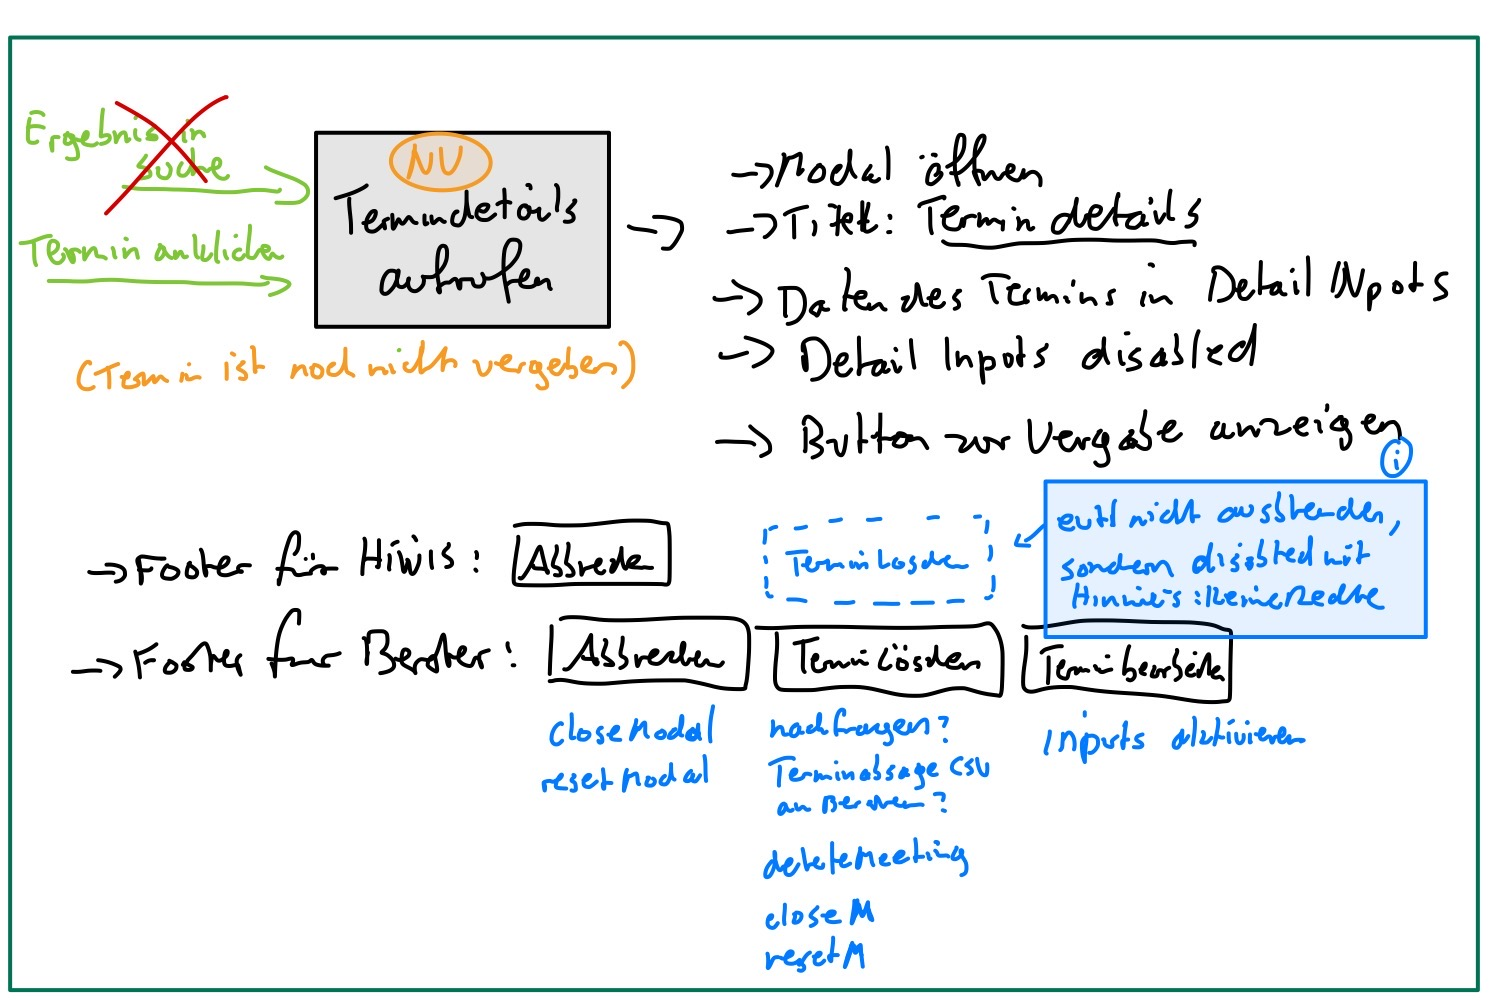
\includegraphics[width=0.9\textwidth]{flow_termin_aufrufen_unvergeben.jpeg}
\end{figure}

Die grünen Pfeile links oben beschreiben, auf welchem Weg die Nutzenden diesen
Workflow anstoßen können. Die Detailansicht eines vergebenen Termins kann in
diesem Fall auf zwei verschiedenen Wegen geöffnet werden. Entweder klickt ein
Nutzender auf einen Termin in der Monatsübersicht oder er klickt auf ein
Suchergebnis in der Ergebnisliste der Suche nach Teilnehmenden. Im rechten
oberen Teil des Diagramms wird stichpunktartig festgehalten, welche
Teilschritte notwendig sind, um die Termindetails sinnvoll darstellen zu können:
Zunächst muss das \gls{Modal} über dem bestehenden Bildschirminhalt
eingeblendet werden. Im nächsten Schritt muss der Titel des Modals angepasst
werden. Der Standardtitel \textit{Termin erstellen} macht in diesem Kontext
keinen Sinn, da der Termin bereits existiert. Daher wird der Titel des Modals
in diesem Fall auf \textit{Termindetails} geändert. Im weiteren Verlauf müssen
die Daten des Termins (Datum, Uhrzeit, Titel) in die entsprechenden Input
Felder geladen werden. Diese Input Felder sollen als \textit{disabled}
dargestellt werden. Das bedeutet, dass man den eingetragenen Inhalt lesen, ihn
jedoch nicht bearbeiten kann. Ein bereits an einen Kunden vergebener Termin
kann nicht bearbeitet werden, solange der Datensatz des Kunden nicht entfernt
wurde. So soll vermieden werden, dass beispielsweise das Datum des
Beratungstermins nachträglich geändert wird, ohne dass der Kunde darüber
informiert wird. Hier wird den Nutzenden also bewusst die Funktionalität des
nachträglichen Änderns verboten, um keine Missverständnisse in der
Kundenkommunikation aufkommen zu lassen. Sollte tatsächlich einmal das Datum
eines Beratungstermins verändert werden, muss der Kundendatensatz zunächst
entfernt und dann, nach dem Anpassen des Datums neu hinzugefügt werden. Dies
hat den Vorteil, dass die entsprechenden Informationsmails (Terminabsage, Neue
Terminbestätigung) korrekt an den Kunden und den Beratenden gesendet werden und
somit für beide Parteien nachvollziehbar ist, an welchem Datum der Termin nun
tatsächlich stattfinden soll.

\begin{figure}[H]
    \caption{Verschiedene Bereiche des Modals mit Kontrollelementen.}
    \centering
    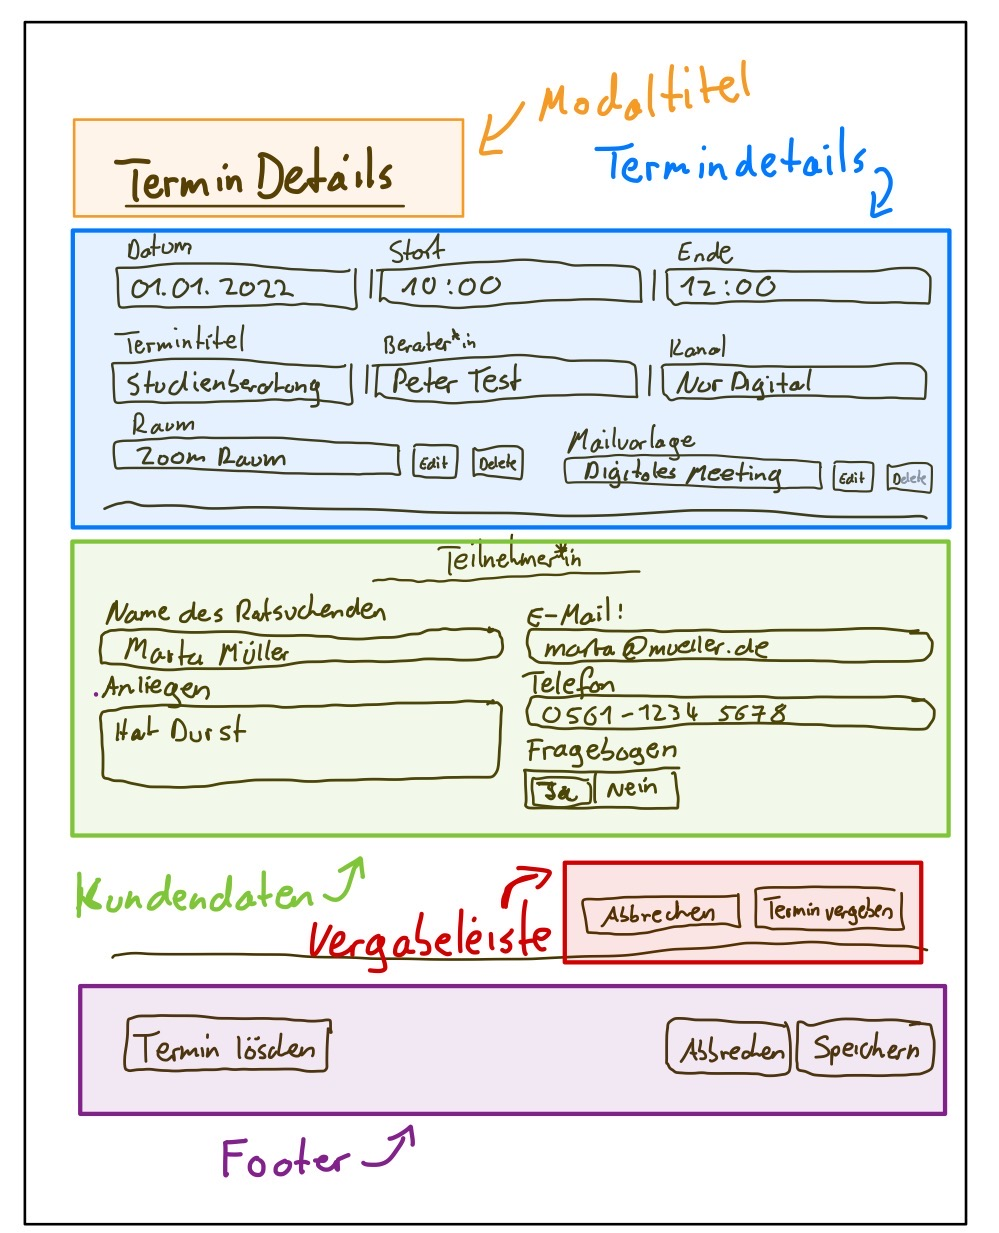
\includegraphics[width=0.9\textwidth]{doodle_modal_overview.jpeg}
\end{figure}

Im unteren Teil des Diagramms wird durch kleine Skizzen festgehalten, welche
Kontrollelemente den Nutzenden im Workflow zur Verfügung stehen. Die
\textit{Vergabeleiste} bezeichnet den Bereich, in dem Buttons zum Interagieren
mit den Kundendaten dargestellt werden. In diesem Fall ist lediglich der Button
\textit{Kundendaten löschen} sichtbar. Ein nachträgliches Bearbeiten der
Kundendaten soll nicht möglich sein, da auch hier inkonsistente Status beim
Versand der Mails an den Kunden entstehen könnten. Wird beispielsweise die
Mailadresse des Kunden geändert, nachdem er für den Versand eines
Feedback-Fragebogens eingetragen wurde, kann der Link für den Fragebogen nicht
mehr an die korrekte Adresse verschickt werden. Diese Problematik wird im
Diagramm grafisch durch die orangene Infobox am rechten Rand verdeutlicht.
Schlussendlich wird im Diagramm dargestellt, welche Buttons in der Fußleiste
des Modals angezeigt werden sollen. Hier soll lediglich der Button
\textit{Abbrechen} aktiv sein. Über diesen Button wird das Modal ohne Übernahme
von Änderungen geschlossen und ein anderer Termin kann aufgerufen werden. Die
Buttons zum Speichern und Löschen des Termins sollten nicht angeklickt werden
können. Wie bereits erwähnt, soll ein Ändern oder Löschen der Termindaten nur
möglich sein, wenn die verknüpften Kundendaten entfernt wurden. Die Buttons
sollen jedoch nicht vollkommen unsichtbar sein, sondern lediglich ausgegraut
dargestellt werden. Die blaue Box im Diagramm ergänzt, dass in diesem Fall ein
Hinweis angezeigt werden soll, in dem den Nutzenden erklärt wird, dass zunächst
die Kundendaten entfernt werden müssen, bevor diese Buttons wieder genutzt
werden können. Dass die Buttons ausgegraut und mit einem Hinweis dargestellt
werden, soll dazu führen, dass Nutzende eine einheitliche Benutzeroberfläche
vorfinden. Bei dem Versuch, mit den deaktivierten Buttons zu interagieren,
sollen sie automatisch darauf hingewiesen werden, welche Schritte notwendig
sind, um die gewünschte Funktion nutzen zu können. Dies soll dazu beitragen,
dass auch unerfahrene Nutzende schnell und intuitiv verstehen, wie eine
Interaktion mit dem System gedacht ist.

Im Anhang (Kapitel \ref{section:anhang:Sequenzdiagramme}) finden sich alle angefertigten Sequenzdiagramme, die auch weitere Prozesse beschreiben: \textit{Vergebenen
    Termin aufrufen}, \textit{Neuen Termin erstellen} und \textit{Termin an Kunden
    vergeben}.

\section{Details der Implementierung}
Im folgenden Abschnitt soll der Fokus nun auf die technischen Details der
Implementierung gelegt werden. Wesentliche Fragestellungen sind hier: Wie
werden die Nutzungsanforderung in der Praxis umgesetzt? Welche Designpattern
und Softwarekonzepte werden verwendet? Wie werden Schnittstellen zwischen
Frontend und Backend gestaltet? Und über welche Protokolle werden Daten
ausgetauscht? Wichtig ist es, an dieser Stelle wieder im Blick zu behalten,
dass es sich um ein Modul in einer bereits bestehenden Software handelt. Somit
sollten bereits existierende Konzepte und Schnittstellen nach Möglichkeit
wieder verwendet werden. Durch das Aufgreifen bestehender Lösungsstrategien und
Entwurfsmuster wird das gesamte Softwarepaket einheitlich strukturiert und ist
somit leichter zu warten. Gleichzeitig müssen einige Funktionen nicht von Grund
auf neu implementiert werden, somit kann Zeit und Arbeit in diesem Prozess
erspart werden \cite{wiederverwSoftware}. Im Folgenden werden einige
Designentscheidungen, Grafiken und Codeschnipsel präsentiert, um einen groben
Einblick in die technische Umsetzung zu erlauben. Der vollständige Sourcecode,
sowie alle Commits zur Programmierung dieses Moduls sind im entsprechenden
GitHub Repository einzusehen. Weitere Details dazu im Anhang unter Abschnitt
\ref{section:stubegru-refs}.

\subsection*{Die Klasse \code{Meeting}}
Die eigentlichen Datenmodelle, mit denen in dem Modul zur Terminvereinbarung
gearbeitet wird, sind relativ simpel gehalten. Es gibt drei relevante Typen von
Datensätzen: Termine, Mailtemplates und Beratungsräume. Die Datensätze, die
einen Termin beschreiben, enthalten außerdem auch Informationen über den
Ratsuchenden, der diesen Termin gebucht hat. Diese Datensätze werden im
Folgenden als \code{Meeting} bezeichnet und sollen anhand eines \gls{UML}
Diagramms detailliert veranschaulicht werden.

\begin{figure}[H]
    \caption{UML Diagramm der Klasse Meeting. Stellt alle Methoden und Eigenschaften eines Objektes dar, das einen Termin repräsentiert.}
    \centering
    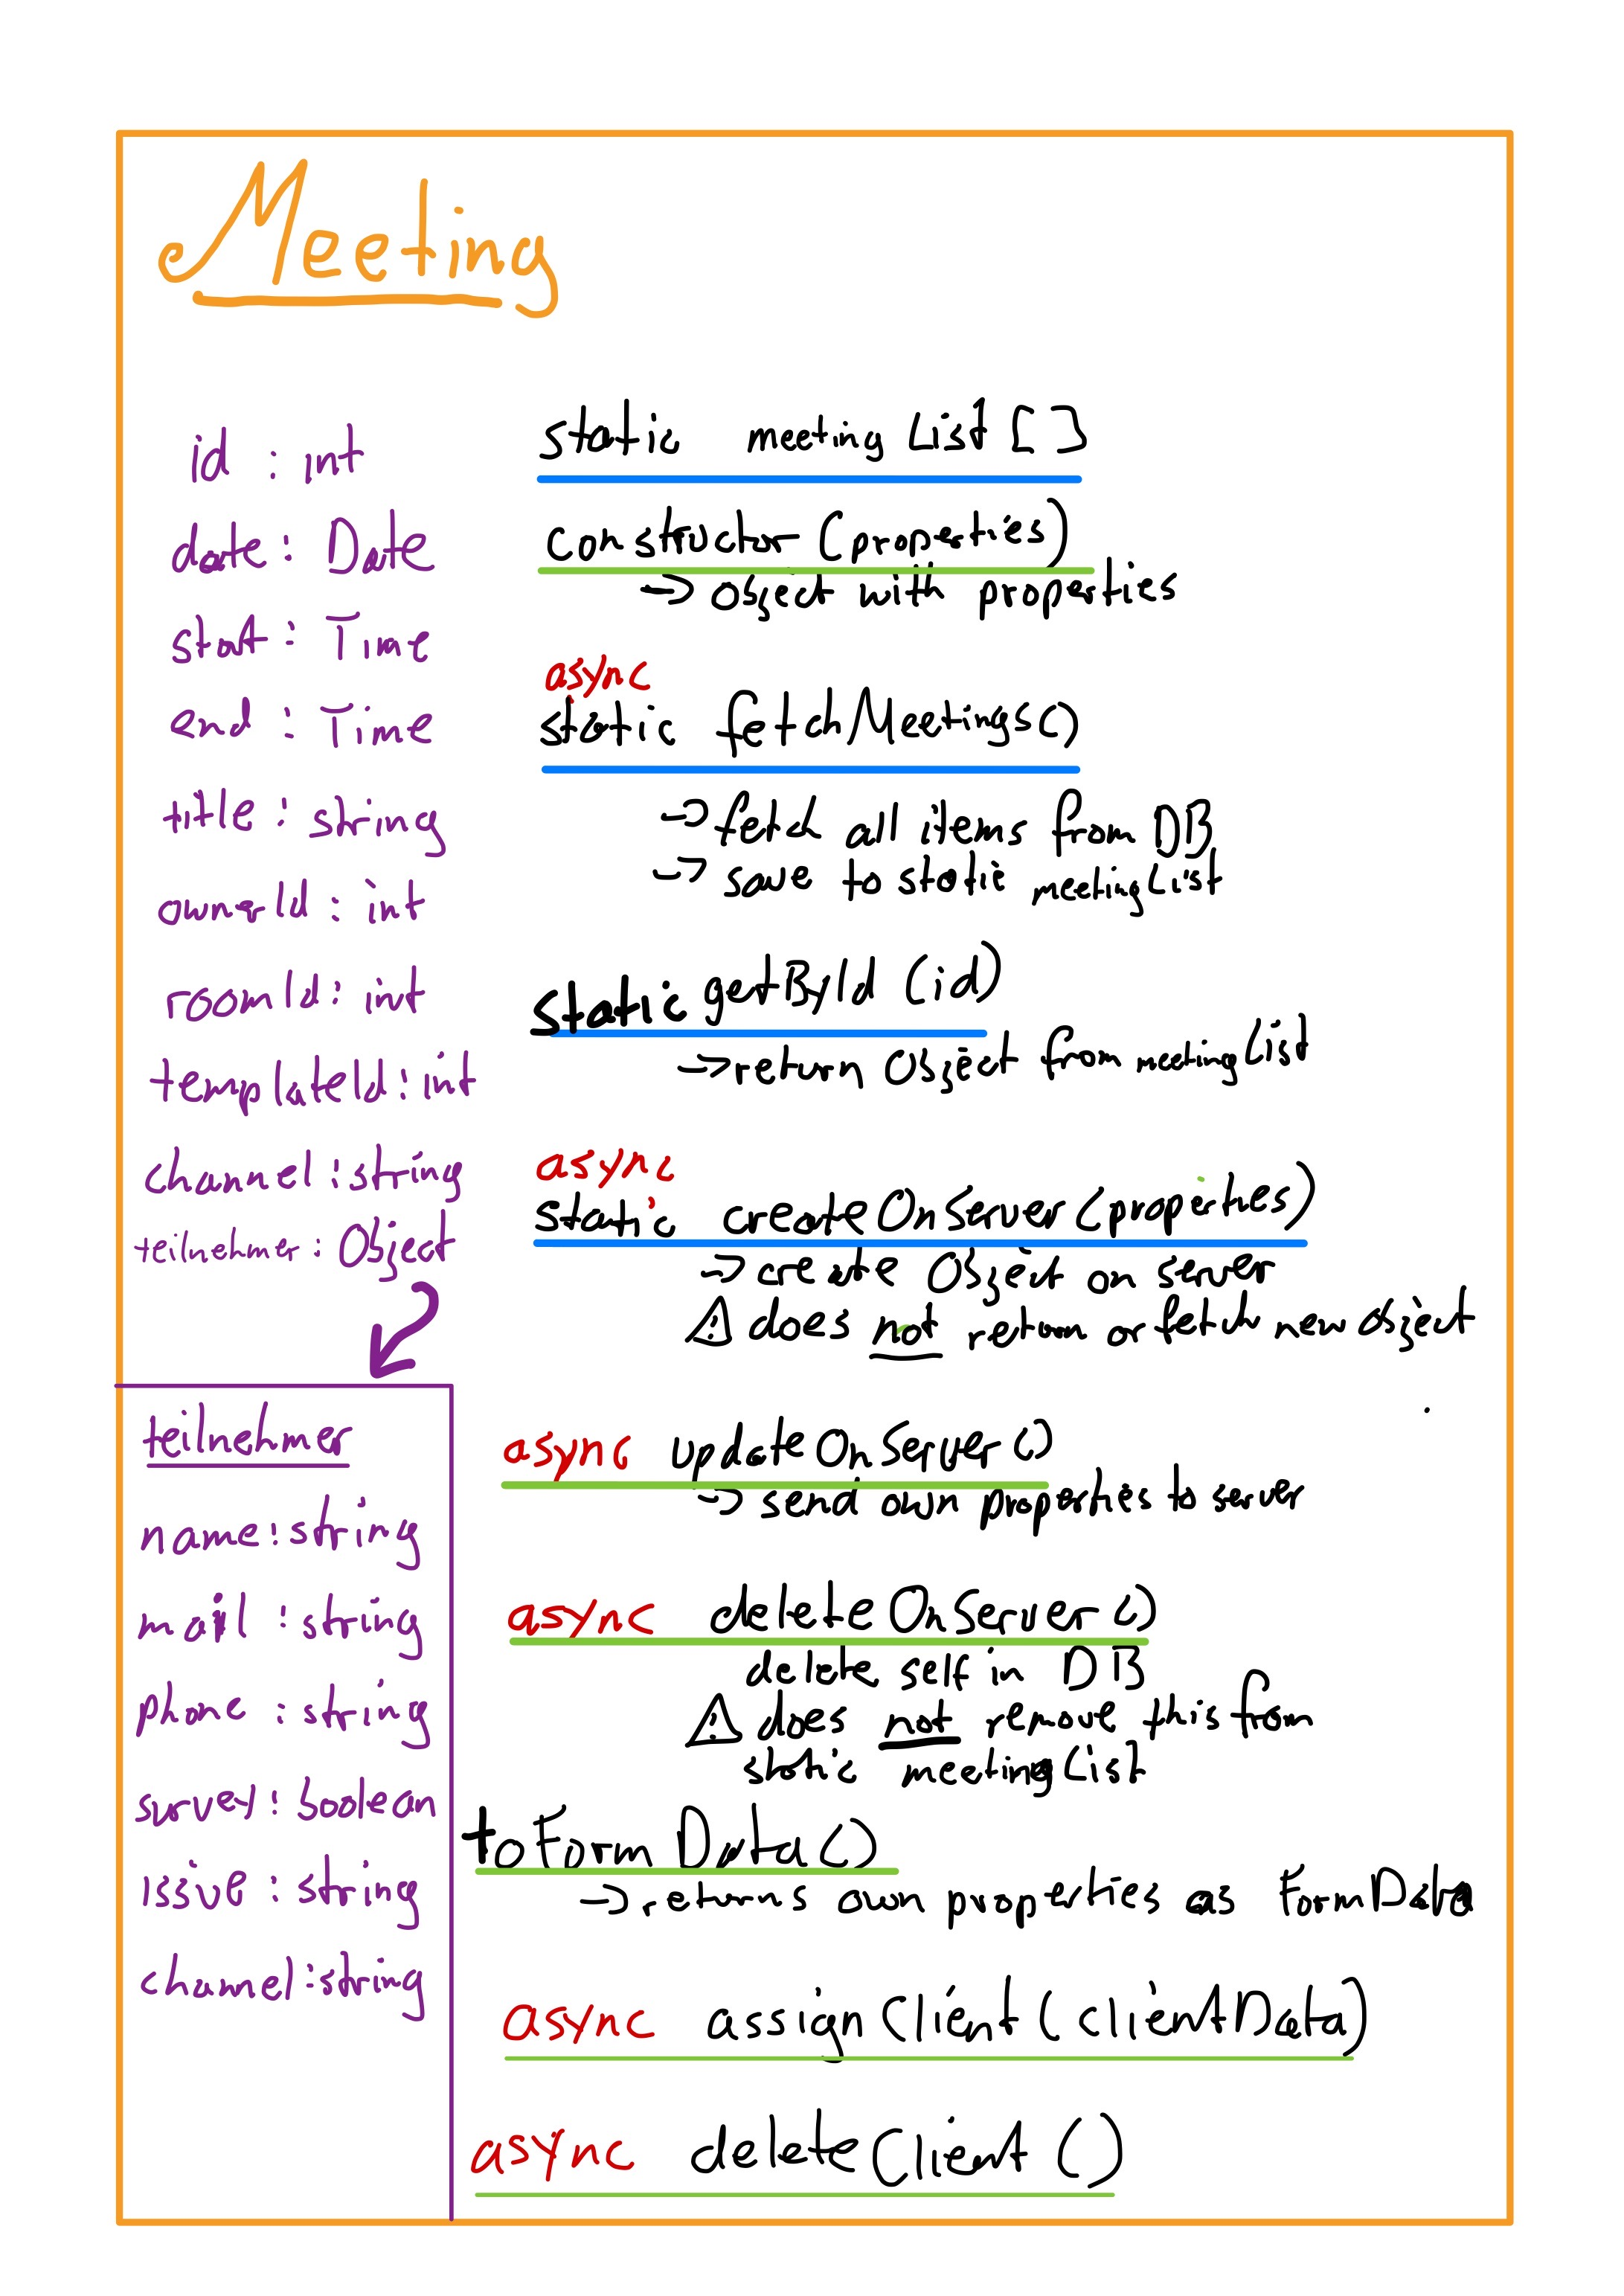
\includegraphics[width=0.9\textwidth]{uml_meeting.jpeg}
\end{figure}

Die Klasse \code{Meeting} stellt zunächst einige statische Eigenschaften und
Methoden zur Verfügung. Das Array \code{meetingList} enthält zur Laufzeit alle
aktuell bekannten Termine in einer unsortierten Liste. Durch die statische
Funktion \code{fetchMeetings()} werden alle Datensätze aus der Datenbank
geladen und in der \code{meetingList} gespeichert. Über die Funktion
\code{getById()} kann ein bestimmtes Meeting aus der \code{meetingList}
angesprochen werden. Die weiteren Funktionen dienen dazu, die Eigenschaften
eines Meetings an das Backend zu senden, um die neuen Werte in der Datenbank zu
speichern oder zu löschen. Die statische Methode
\code{createOnServer(properties)} sendet die Daten eines neuen Meetings an den
Server. Diese Methode erstellt bewusst keine neue Instanz vom Typ
\code{Meeting}, da es keinen Sinn macht, ein Meeting Objekt zu verwenden,
solange der Server dieses Meeting noch gar nicht kennt. Im Anschluss an die
\code{createOnServer(properties)} Methode sollte stets die Methode
\code{fetchMeetings()} aufgerufen werden, um auf das neu erstellte Meeting
zugreifen zu können. Die Funktion \code{updateServer()} wird auf einem
bestehenden Objekt vom Typ \code{Meeting} aufgerufen und sendet die aktuellen
lokalen Eigenschaften an den Server. Hierbei wird die Funktion
\code{toFormData()} verwendet, um die Eigenschaften des Objektes in das
passende Format zu bringen. Die so aufbereiteten Daten werden über den
asynchronen Aufruf der \gls{fetch-api} mit einer Http Request an das
entsprechende Php Skript auf dem Server gesendet.

\lstinputlisting[style=ES6, caption=Senden von lokalen Änderungen eines Meetings an den Server]{listings/updateOnServer.js}

Über die Methode \code{deleteOnServer()} kann ein bestehendes Meeting auf dem Server gelöscht werden. Durch einen anschließenden Aufruf von \code{fetchMeetings()} wird das Meeting dann auch in der lokalen \code{meetingList} gelöscht. Außerdem stellt ein Objekt vom Typ \code{Meeting} noch zwei Methoden zur Verfügung, um Kundendaten zu verknüpfen, beziehungsweise zu löschen. Diese Funktionen stoßen in den jeweiligen Php Skripten auf dem Server weitere Workflows an, wie beispielsweise das Versenden einer Bestätigungsmail an die ratsuchende Person.

\lstinputlisting[style=PHP-colored, caption=Php Skript zum Erstellen eines neuen Meetings in der Datenbank]{listings/save_meeting.Php}



\subsection*{Vergebenen Beratungstermin aufrufen}

In Kapitel \ref{subsection:sequenceDiagrams} wurden exemplarisch alle
Teilschritte erklärt, die nötig sind, um einen bereits vergebenen
Beratungstermin aufzurufen und in der Detailansicht darzustellen. Für jeden
dieser einzelnen Schritte wurde eine entsprechende Funktion in der Klasse
\code{CalendarModal} implementiert. Die Funktion
\code{setModalVisible(isVisible)} kann beispielsweise aufgerufen werden, um das
Modal ein- oder auszublenden. Die Klasse \code{CalendarController} verwendet
nun all diese Funktionen und bildet so den kompletten beschriebenen Workflow
Schritt für Schritt ab. Das folgende Listing beschreibt den Ablauf aller
einzelnen Schritte durch den sequenziellen Aufruf der einzelnen Funktionen:

\lstinputlisting[style=ES6, caption=Öffnen der Detailansicht eines vergebenen Beratungstermins]{listings/openAssignedMeeting.js}




\subsection*{Monatsansicht mit fullcalendar darstellen}

Als abschließendes Beispiel der konkreten Implementierung wird die Klasse
\code{CalendarView} vorgestellt. Diese ist für das Darstellen der
Terminübersicht zuständig. An dieser Stelle wird die Javascript Bibliothek
\gls{fullcalendar} verwendet, um den Aufbau der Monatsansicht deutlich zu vereinfachen. Die Klasse \code{CalendarView}
referenziert auf eine Instanz vom Typ \code{FullCalendar} und kann darüber die
wichtigsten Funktionen zum Löschen und Hinzufügen weiterer Termine aufrufen. Im
folgenden Listing wird die Funktion \code{addMeetings(meetingList)} gezeigt.
Diese Funktion wird vom \code{CalendarController} aufgerufen und bekommt als
Parameter eine Liste von Meetings übergeben. Aus den übergebenen Objekten vom
Typ \code{Meeting} werden zunächst Objekte generiert, die alle Eigenschaften
erhalten, welche die fullcalendar Bibliothek benötigt, um die Termine
in der Übersicht korrekt anzeigen zu können. Die so erstellten Datensätze
werden anschließend in \textit{freie Termine} und \textit{vergebene Termine}
sortiert. Über die Funktion \code{fullCalendar.addEventSource(eventSource)}
werden die Listen mit den freien und den vergebenen Terminen hinzugefügt. Über
den weiteren Parameter \code{color} wird in diesem Fall die farbliche
Darstellung der Termine (grün = frei, rot = vergeben) in der Monatsübersicht gesteuert.

\lstinputlisting[style=ES6, caption=Hinzufügen von Terminen in die Monatsübersicht von fullcalendar]{listings/addMeetings.js}